\chapter{Discussion}
Please tell more about conclusion and how to the next work of this study.

\section{Andri Fajar Sunandhar / 1164065}
\subsection{Teori}
\begin{enumerate}
\item Mengapa file suara harus dilakukan MFCC, dilengkapi dengan ilustrasi atau gambar.
\par Mel Frequency Cepstral Coefficients (MFCC) merupakan koefisien yang merepresentasikan audio. Sehingga diharuskannya melakukan MFCC kepada objek suara atau audio agar suara dapat berubah atau diubah ke dalam bentuk data matrix dimana telah dilakukan ekstraksi oleh MFCC kemudian direalisasikan sebagai data matrix. Ilustrasinya bisa dilihat pada gambar berikut  \ref{no1}.
	\begin{figure}[ht]
	\centerline{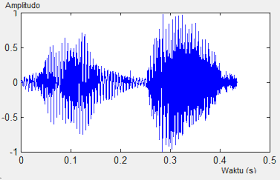
\includegraphics[width=0.5\textwidth]{figures/chapter6/no1.png}}
	\caption{Gambar MFCC.}
	\label{no1}
	\end{figure}

\item Konsep dasar Neural Network, dilengkapi dengan ilustrasi atau gambar.
\par Neural Network merupakan kategori ilmu Soft Computing. Neural Network sebenarnya mengadopsi dari kemampuan otak manusia yang mampu memberikan stimulasi/rangsangan, melakukan proses, dan memberikan output. Output diperoleh dari variasi stimulasi dan proses yang terjadi di dalam otak manusia. Kemampuan manusia dalam memproses informasi merupakan hasil kompleksitas proses di dalam otak. Misalnya, yang terjadi pada anak-anak, mereka mampu belajar untuk melakukan pengenalan meskipun mereka tidak mengetahui algoritma apa yang digunakan.  Ilustrasinya bisa dilihat pada gambar berikut   \ref{no2}.
	\begin{figure}[ht]
	\centerline{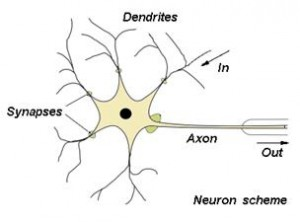
\includegraphics[width=0.5\textwidth]{figures/chapter6/no2.jpg}}
	\caption{Gambar Neural Network.}
	\label{no2}
	\end{figure}

\item Konsep pembobotan Neural Network, dilengkapi dengan ilustrasi atau gambar.
\par Sebuah Neural Network dikonfigurasi untuk aplikasi tertentu, seperti pengenalan pola atau klasifikasi data. Terjadi penglibatan dalam penyesuaian koneksi sinaptik yang ada antara neuron ketika melakukan penyempurnaan dengan proses pembelajaran. Penyesuaian nilai bobot yang ada pada tiap konektivitas baik dari input, neuron maupun output disinkronkan dengan penyesuaian koneksi sinaptik antar neuron itu sendiri.  Ilustrasinya bisa dilihat pada gambar berikut  \ref{no3}.
	\begin{figure}[ht]
	\centerline{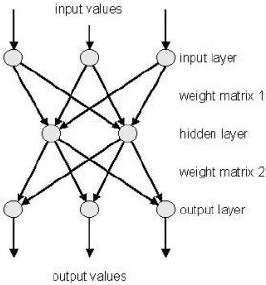
\includegraphics[width=0.5\textwidth]{figures/chapter6/no3.jpg}}
	\caption{Gambari Pembobotan neural network.}
	\label{no3}
	\end{figure}

\item Konsep fungsi aktifasi dalam Neural Network, dilengkapi dengan ilustrasi atau gambar
\par Operasi matematik yang dikenakan pada sinyal output y. Sehingga fungsi ini akan digunakan untuk pengaktifan dan juga penonaktifan neuron. Ilustrasinya bisa dilihat pada gambar berikut  \ref{no4}.
	\begin{figure}[ht]
	\centerline{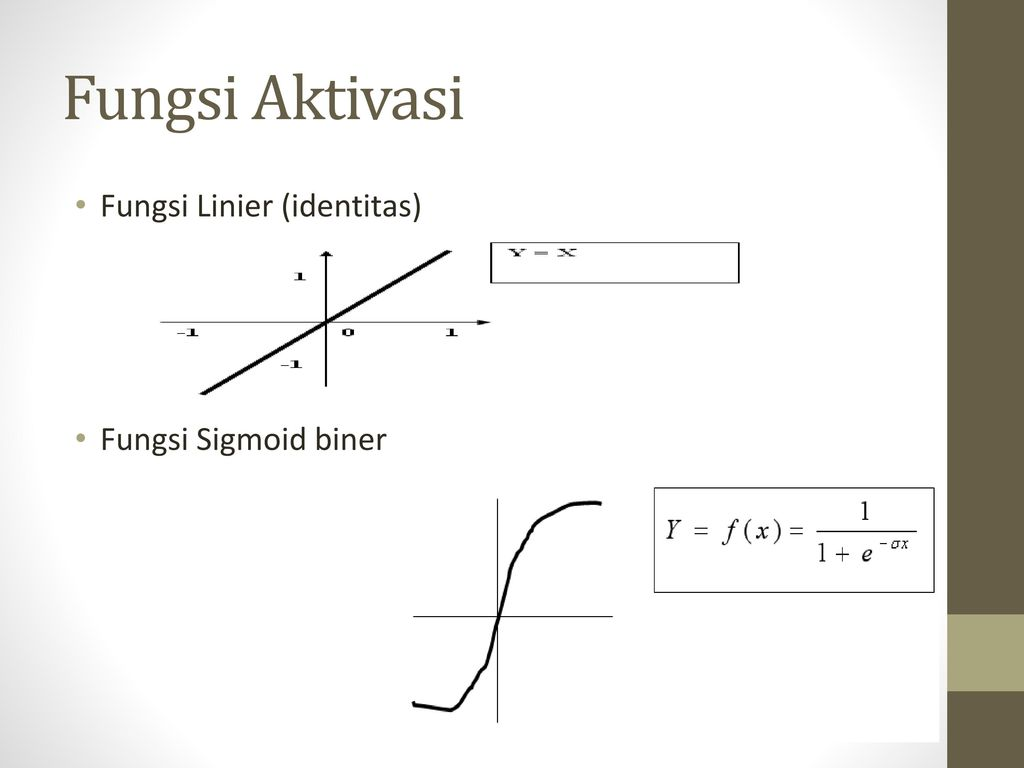
\includegraphics[width=0.5\textwidth]{figures/chapter6/no4.jpg}}
	\caption{Gambar Aktivitas neural network.}
	\label{no4}
	\end{figure}

\item Cara membaca hasil plot dari MFCC, dilengkapi dengan ilustrasi atau gambar.
\par Nanti akan ada outputan berbentuk grafik. Ada 3 dimensi atau sumbu. Dimana untuk sumbu x merupakan waktu, sedangkan sumbu y merupakan frekuensi dari suara yang dihasilkan dalam bentu Hz. Sedangkan pada bagian tengah atau sumbu z merupakan power atau kekuatan dari lagu atau suara atau desibel yang dihasilkan. Untuk melihat penjelasan dari warna pada gambar yang di tengah, maka kita harus mendownload gambar nya terlebih dahuhulu. Untuk warna biru itu merupakan suara rendah, yang merah merupakan tinggi dan daya frekuensi nya berada pada nilai yang rendah karena bass bekerja pada suara yang rendah. Tidak selalu tergantung pada warna untuk menentukan nilai atau frekuensinya. Tetapi pada jenis lagu yang dugunakan.  Ilustrasinya bisa dilihat pada gambar berikut \ref{no5m}
	\begin{figure}[ht]
	\centerline{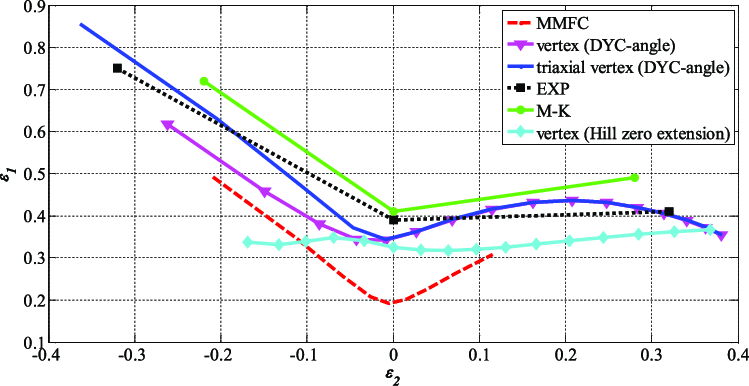
\includegraphics[width=0.5\textwidth]{figures/chapter6/no5.png}}
	\caption{Gambar Plot dari MFCC.}
	\label{no5m}
	\end{figure}

\item Apa itu One-Hot Encoding, dilengkapi dengan ilustrasi atau gambar.
\par One-Hot Encoding adalah sekelompok bit yang kombinasi hukumnya hanya terdiri dari bit dengan bit tinggi (1) dan bit lainnya rendah (0). Implementasi serupa di mana semua bit '1' kecuali satu '0' kadang-kadang disebut one-cold. Dalam statistik, variabel dummy mewakili teknik serupa untuk mewakili data kategorikal.  Ilustrasinya bisa dilihat pada gambar berikut  \ref{no6}.
	\begin{figure}[ht]
	\centerline{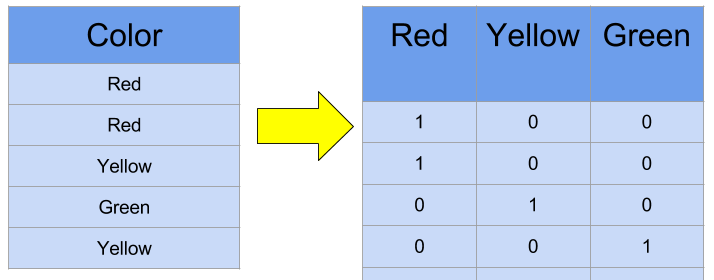
\includegraphics[width=0.5\textwidth]{figures/chapter6/no6.png}}
	\caption{Gambar One-hot Encoding.}
	\label{no6}
	\end{figure}

\item Fungsi dari np.unique dan to.categorical, dilengkapi dengan ilustrasi atau gambar.
\par Np.unique Berfungsi untuk menemukan elemen unik array.  Ilustrasinya bisa dilihat pada gambar berikut  \ref{no7a}.
Ada tiga output opsional selain elemen unik:
	\begin{itemize}
	\item Indeks array input yang memberikan nilai unik
	\item Indeks array unik yang merekonstruksi array input
	\item Berapa kali setiap nilai unik muncul dalam array input
	\end{itemize}
		\begin{figure}[ht]
		\centerline{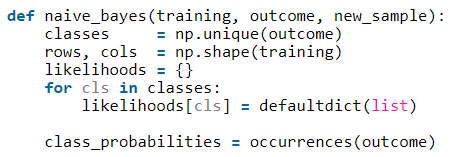
\includegraphics[width=0.5\textwidth]{figures/chapter6/no7a.png}}
		\caption{Gambar np.unique.}
		\label{no7a}
		\end{figure}

\par To.categorical Berfungsi untuk menemukan elemen unik array.  Ilustrasinya bisa dilihat pada gambar berikut  \ref{no7b}.
	\begin{figure}[ht]
	\centerline{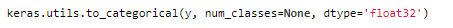
\includegraphics[width=0.5\textwidth]{figures/chapter6/no7b.png}}
	\caption{Gambar to.categorical.}
	\label{no7b}
	\end{figure}

\item Fungsi dari Sequential, dilengkapi dengan ilustrasi atau gambar.
\par Sebuah jenis model yang digunakan dalam perhitungan ataupun code program yang direalisasikan. Neural Networks Sequential membangun fitur tingkat tinggi melalui lapisannya yang berurutan. Sequential juga merupakan proses dimana membandingkan setiap elemen larik satu per satu secara beruntun, mulai dari elemen pertama, sampai dengan elemen terakhir atau elemen yang dicari sudah ditemukanl.  Ilustrasinya bisa dilihat pada gambar berikut  \ref{no8}.
	\begin{figure}[ht]
	\centerline{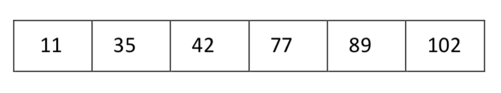
\includegraphics[width=0.5\textwidth]{figures/chapter6/no8.png}}
	\caption{Gambar Sequential.}
	\label{no8}
	\end{figure}
\end{enumerate}